
\documentclass[10pt,twocolumn]{witseiepaper}
%
% All KJN's macros and goodies (some shameless borrowing from SPL)
\usepackage{KJN}
\usepackage[super]{nth}
\usepackage{subcaption}
\usepackage{listings}
\usepackage{amsmath}
\usepackage{epstopdf}
\usepackage{xcolor}
\usepackage{textcomp}
\usepackage{listings}
\usepackage{alltt}
\usepackage{matlab-prettifier}
\usepackage{graphicx}
\usepackage{changes}
\usepackage{makecell}
\usepackage{verbatim}
\usepackage{algorithm,algpseudocode}
\usepackage{balance}
\usepackage{pdfpages}
\usepackage{makecell}
\usepackage{color} %red, green, blue, yellow, cyan, magenta, black, white
\definecolor{mygreen}{RGB}{28,172,0} % color values Red, Green, Blue
\definecolor{mylilas}{RGB}{170,55,241}
%\usepackage{flafter}

%\usepackage[parfill]{parskip}
%\usepackage{titlesec}
%
%\titleformat{\subsubsection}
%{\normalfont\normalsize\itshape}{\thesubsubsection}{1em}{}
%\titlespacing*{\subsubsection}{0pt}{3.25ex plus 1ex minus .2ex}{0ex plus .2ex}

\lstset{language=Matlab, % Set colour for matlab code
	breaklines=true,%
	morekeywords={matlab2tikz},
	keywordstyle=\color{blue},%
	morekeywords=[2]{1}, keywordstyle=[2]{\color{black}},
	identifierstyle=\color{black},%
	stringstyle=\color{mylilas},
	commentstyle=\color{mygreen},%
	showstringspaces=false,%without this there will be a symbol in the places where there is a space
	numbers=left,%
	numberstyle={\tiny \color{black}},% size of the numbers
	numbersep=9pt, % this defines how far the numbers are from the text
	emph=[1]{for,end,break},emphstyle=[1]\color{red}, %some words to emphasise
	%emph=[2]{word1,word2}, emphstyle=[2]{style},    
}
%
% PDF Info
%
\ifpdf
\pdfinfo{
/Title (INSTRUCTIONS AND STYLE GUIDELINES FOR THE PREPARATION OF FINAL YEAR LABORATORY PROJECT PAPERS : 2005 VERSION)
/Author (Ken J Nixon)
/CreationDate (D:200309251200)
/ModDate (D:200510121530)
/Subject (ELEN417/455 Paper Format, 2005)
/Keywords (ELEN417, ELEN455, paper, instructions, style guidelines, laboratory project)
}
\fi

%%%%%%%%%%%%%%%%%%%%%%%%%%%%%%%%%%%%%%%%%%%%%%%%%%%%%%%%%%%%%%%%%%%%%%%%%%%%%%%
\begin{document}


\title{TITLE}

\author{Sasha Berkiwitz (818737) \& Lara Timm (704157)
\thanks{School of Electrical \& Information Engineering, University of the
Witwatersrand, Private Bag 3, 2050, Johannesburg, South Africa}
}


%%%%%%%%%%%%%%%%%%%%%%%%%%%%%%%%%%%%%%%%%%%%%%%%%%%%%%%%%%%%%%%%%%%%%%%%%%%%%%%
%
\abstract{}

\keywords{}

\maketitle
%\thispagestyle{empty}
\pagestyle{plain}
\setcounter{page}{1}


%%%%%%%%%%%%%%%%%%%%%%%%%%%%%%%%%%%%%%%%%%%%%%%%%%%%%%%%%%%%%%%%%%%%%%%%%%%%%%%
\section{INTRODUCTION}

File Transfer Protocol (FTP) is a protocol which is used  to transfer files between two hosts over a TCP or IP network~\cite{FTPbeginners}. In it's operation FTP makes use of two TCP connections, a control connection and a data connection. The control connection, used to send control information, is opened and remains open throughout the duration of the user session~\cite{topDownApproach6th}. The data connection is non-persistent; a new data connection is established for each new file transfer~\cite{topDownApproach6th}. The main objectives of FTP include the promotion of file sharing, to encourage the use of remote computers, to shield users from variations in file storage systems among hosts and to ensure reliable and efficient data transfer~\cite{rfc959}. 

%Using the python programming language as well as basic socket methods, a File Transfer Application is designed and tested. Additionally, a basic FTP User Interface (UI) is developed to interact with the remote FTP server in an intuitive way.

Detailed within the sections below are a overview of the implemented system and its command/reply messaging exchange, a working description of the system and code base,the results of system testing and a critical analysis thereof. Also included is the division of work between the project partners.

%%%%%%%%%%%%%%%%%%%%%%%%%%%%%%%%%%%%%%%%%%%%%%%%%%%%%%%%%%%%%%%%%%%%%%%%%%%%%%%
\section{SYSTEM DESCRIPTION} 

An FTP client and server pair has been designed and implemented as per RFC~959 specifications~\cite{rfc959}. By implementing the system in such a way, both the server and client are compatible standardised servers and clients. A limitation of the system is that it is not designed for any platform other than the Windows OS.

\subsection{FTP Server}

The FTP server is hosted locally, and can be accessed by an FTP client which is either connecting from the hosts computer, or from a computer running on the same Local Area Network (LAN) via the server's public IP address. 

In order to provide unique user experience, the server maintains a user repository, within the servers local file system, for each registered client. To gain access to their remote repository, the user must be successfully authenticated using their unique username and password combination. Clients trying to connect without a registered username and password are not permitted to access the server file system.

The server is implemented in accordance with the RFC~959 specification. The implemented features of the system go beyond those of the minimum requirements set out by the standard, improving the system's general functionality and usability. Following RFC~959 allows for the server to be accessed by not only the designed client but also standardised FTP clients. 

To allow for more than one client to be connected to the server at a time, the server program is multithreaded. Each new client connection is handled by a separate thread, and up to five simultaneous connections can be established by FTP clients. 

To communicate file, system and transfer status to the client, the server makes use of a number of RFC~959 specified reply codes. These codes enable the client to detect errors and react accordingly. Further discussion of this process can be found in Section~\ref{sec:command/reply}

\subsubsection*{Unimplemented features: }
In accordance with the RFC~959 minimum requirements, the default structure and file transmission mode for exchange should be implemented. Functionality for Record and Page structures, as well as for Block and Compressed transmission modes were not implemented. The project group deemed theses features unnecessary as standard FTP clients would be able to transmit in File structure and Stream transmission modes which are default.

\subsection{FTP Client}

The FTP client is composed of two working parts, a Graphical User Interface (GUI) and a logical FTP client. The user interacts with the GUI which instructs the FTP client to interact with the FTP server. In this way the interface is separated from the logic layer, following the separation of concerns principle.

\subsubsection{Client Logic} $     $

The FTP client is hosted locally and can connect to a server hosted either locally (on the client's computer) or over a LAN connection. To connect to the server, the client must know the public IP address and port on which the server is listening for a connection. These parameters are input to the GUI described in Section~\ref{GUI}.

The responsibility of the FTP client is to interact with the server in a manner in which the server understands. The client translates the raw data received from the GUI by formatting it to comply with the RFC~959 specification. In this way, the client can not only interact with the designed server, but also  with a range of standard FTP servers.

It is the responsibility of the client to handle errors that are not relevant to the server. Such errors include: trying to upload a file that doesn't exist in the clients working directory and handling errors to do with incorrect formatting of client commands. Although these checks are implemented in the server program, the client will most often prevent these user errors from occurring.

\subsubsection{Client Interface: }\label{GUI} $     $
%Sash%%%%%%%%%%%%%%%

%The FTP client is handled by a simple GUI. 

%input params (name pass addr IP)

%can view and nav both file systems

% can upload from local or dl from remote - file saved to current working dir

%can delete files/folders (folder removes all contents) %%MAKE POPUP TO ASK IF SURE%??
%can make folders local and remote?

%client can input custom commands if necessary.

%client disconnects by?


\subsubsection*{Unimplemented features: } 
In accordance with the server implementation, the client is only capable of handling the File structure and Stream mode of data transmission as specified in the minimum RFC~959 requirements.

%Sash%%%%%%%%%%%%%%%
%cannot make new files on either side, copy paste etc. 
%cannot remane files/folders on either side
%cannot edit files on either side


%%%%%%%%%%%%%%%%%%%%%%%%%%%%%%%%%%%%%%%%%%%%%%%%%%%%%%%%%%%%%%%%%%%%%%%%%%%%%%%
\section{FTP COMMAND/REPLY OVERVIEW}\label{sec:command/reply}

The format of replies to FTP commands are designed to make sure that requests and actions are well synchronized when transferring files, and to ensure the client informed about the status of the server at all times~\cite{rfc959}. There are 5 categories of FTP replies, characterised by the first digit of the three digit reply code~\cite{rfc959}. 

The categories are: 

\textbf{1**	Positive Preliminary reply:} 
Requested action initiated, expect reply before sending new command.

\textbf{2**	Positive Completion reply:} 
Requested action completed, new command can be sent.

\textbf{3**   Positive Intermediate reply:} 
Command received, server waiting for further information.

\textbf{4**   Transient Negative Completion reply:} 
Command not accepted, action did not take place. Error is temporary and action may be requested again.

\textbf{5**   Permanent Negative Completion reply:} 
Command not accepted, action did not take place. User discouraged from repeating same request.

In the designed file transfer application, at least one reply was implemented from each category. A list of the implemented commands and their associated server responses are detailed in Appendix~\ref{sec:comm-replyTable}.

%%%%%%%%%%%%%%%%%%%%%%%%%%%%%%%%%%%%%%%%%%%%%%%%%%%%%%%%%%%%%%%%%%%%%%%%%%%%%%%
\section{DETAILED FEATURE IMPLEMENTATION} % talk about details of how the complex functions work

\subsection{Client Authentication}

\subsection{Directory Traversal}

\subsection{Data Connection Initiation}

\subsection{File Transfer}

\subsection{Miscellaneous}



%\begin{figure}[h]
%	\centering
%	\includegraphics[width=0.9\columnwidth]{collisions.png}
%	\caption{Illustration of the collision relationships that exist between game objects. Arrowheads indicate damage dealt.}
%	\raggedright
%	\label{fig:collisions}
%\end{figure}

%%%%%%%%%%%%%%%%%%%%%%%%%%%%%%%%%%%%%%%%%%%%%%%%%%%%%%%%%%%%%%%%%%%%%%%%%%%%%%%
\section{DIVISION OF WORK}

%%%%%%%%%%%%%%%%%%%%%%%%%%%%%%%%%%%%%%%%%%%%%%%%%%%%%%%%%%%%%%%%%%%%%%%%%%%%%%%
\section{RESULTS}\label{results}

To test the system fully, testing of all functionally on the client and server side is required. This must therefore include testing the FTP client with the implemented FTP server as well as with a standard FTP server. Additionally, the designed FTP server should be tested with a standard FTP client, namely FileZilla.

Using the Wireshark platform, a copy of every packet of data sent over a wired or wireless internet connection is recorded. Wireshark is used to test the developed file transfer application.

Functionality testing begins with ensuring the client can connect. After the server confirms that a control connection has been made, the user logs in with their username and password. The client can then navigate around their own remote file repository. 

To upload or download files, the file type is set, a data connection is established and the file is transmitted or received. The client can create directories, as well as delete. Files however, cannot be created;  only deleted.

Using Wireshark, these interactions were logged. Appendix~\ref{sec:wireshark} contains screenshots of the described interactions. 

Figure ~\ref{fig:WitsWS1} yuyguihlkjhgfghjk
%%%%%%%%%%%%%%%%%%%%%%%%%%%%%%%%%%%%%%%%%%%%%%%%%%%%%%%%%%%%%%%%%%%%%%%%%%%%%%%
\section{CRITICAL ANALYSIS}

%%%%%%%%%%%%%%%%%%%%%%%%%%%%%%%%%%%%%%%%%%%%%%%%%%%%%%%%%%%%%%%%%%%%%%%%%%%%%%%
\section{CODE STRUCTURE}

%%%%%%%%%%%%%%%%%%%%%%%%%%%%%%%%%%%%%%%%%%%%%%%%%%%%%%%%%%%%%%%%%%%%%%%%%%%%%%%
\section{CONCLUSION}


%%%%%%%%%%%%%%%%%%%%%%%%%%%%%%%%%%%%%%%%%%%%%%%%%%%%%%%%%%%%%%%%%%%%%%%%%%%%%%%
%
%\nocite{*}
\bibliographystyle{witseie}
\bibliography{FTPbib}

\newpage
\onecolumn


\begin{appendix}
	
\setcounter{figure}{0} \renewcommand{\thefigure}{A\arabic{figure}}
	
\section{Implemented FTP Commands/Replies} \label{sec:comm-replyTable}

\begin{tabular}{|l|l|l|}
	\hline 
	\textbf{Command} & \textbf{Command Description} & \textbf{Server Replies} \\ 
	\hline 
	USER & \multicolumn{1}{p{6cm}|}
	{\raggedright The username input to the GUI is sent to the server for authentication } &  \multicolumn{1}{p{8.3cm}|}
	{\raggedright 331 User name okay, need password. \\ 332 Need account for login.} \\ 
	\hline 
	PASS & \multicolumn{1}{p{6cm}|}
	{\raggedright The password input to the GUI is sent to the server for authentication} &  \multicolumn{1}{p{8.3cm}|}
	{\raggedright 230 User logged in, proceed. \\ 332 Need account for login. \\ 530 Not logged in. Password invalid.} \\ 
	\hline 
	CWD & \multicolumn{1}{p{6cm}|}
	{\raggedright Changes the working directory on the server. Argument is the name of the directory to change to. } &  \multicolumn{1}{p{8.3cm}|}
	{\raggedright 250 Requested action okay. Working directory changed. \\ 550 Requested action not taken. Directory does not exist.} \\ 
	\hline 
	CDUP & \multicolumn{1}{p{6cm}|}
	{\raggedright Go up one directory on the server. User cannot go further up than their base directory.} &  \multicolumn{1}{p{8.3cm}|}
	{\raggedright 250 Requested action okay. Working directory changed. \\ 550 Requested action not taken. Permission denied.} \\ 
	\hline 
	QUIT & \multicolumn{1}{p{6cm}|}
	{\raggedright Closes the control connection between the client and server.} & 221 Service closing control connection. \\ 
	\hline
	PORT & \multicolumn{1}{p{6cm}|}
	{\raggedright The client specifies a port for the data connection. Arguments are the IP address and port on which the client is listening for a connection.} & 200 Port command successful. \\ 
	\hline 
	PASV & \multicolumn{1}{p{6cm}|}
	{\raggedright Requests that the server listens on an available port for a client data connection. The clients connects to the port specified in the server response.} & 227 Entering passive mode (\textit{IP address}, \textit{Port}) \\ 
	\hline 
	TYPE & \multicolumn{1}{p{6cm}|}
	{\raggedright Specifies the type of the file which is to be uploaded to or downloaded from the server. ASCII and Binary types are implemented.} &  \multicolumn{1}{p{8.3cm}|}
	{\raggedright 200 Switching to Binary mode. \\ 200 Switching to ASCII mode. \\ 504 Command not implemented for that parameter.} \\ 
	\hline 
	STRU & \multicolumn{1}{p{6cm}|}
	{\raggedright Specifies the structure of the file which is to be uploaded to or downloaded from the server.  File structure is implemented. } &  \multicolumn{1}{p{8.3cm}|}
	{\raggedright 200 Switching to File structure mode.  \\ 504 Command not implemented for that parameter.} \\ 
	\hline 
	MODE & \multicolumn{1}{p{6cm}|}
	{\raggedright Specifies the transfer mode of the file which is to be uploaded to or downloaded from the server.  Stream transfer mode is implemented.} &  \multicolumn{1}{p{8.3cm}|}
	{\raggedright 200 Switching to Stream transfer mode.  \\ 504 Command not implemented for that parameter.} \\ 
	\hline 
	RETR & \multicolumn{1}{p{6cm}|}
	{\raggedright A copy of a file existing on the server is sent to the client over a data connection. The command argument is the name of the file to be retrieved.} &  \multicolumn{1}{p{8.3cm}|}
	{\raggedright 150 Opening data connection. \\ 226 Closing data connection. File action successful. \\ 550 Requested action not taken. File unavailable. \\ 451 Requested action aborted: local error in processing. \\ 425 Use PORT or PASV first.} \\ 
	\hline  
	STOR & \multicolumn{1}{p{6cm}|}
	{\raggedright A copy of a file existing on the client's computer is sent to the server over a data connection. The command argument is the name of the file to be stored.} &  \multicolumn{1}{p{8.3cm}|}
	{\raggedright 150 File status okay. Opening data connection. \\ 226 Closing data connection. File action successful. \\ 550 Requested action not taken. File transfer unsuccessful.  \\ 425 Use PORT or PASV first.} \\  
	\hline 
	DELE & \multicolumn{1}{p{6cm}|}
	{\raggedright A specified file is deleted from the server. The argument is the name of the file to be deleted } &  \multicolumn{1}{p{8.3cm}|}
	{\raggedright 250 Requested file action okay, file deleted. \\ 550 Requested action not taken. To delete directory use RMD. \\ 550 Requested action not taken. File does not exist.} \\  
	\hline 
	PWD & \multicolumn{1}{p{6cm}|}
	{\raggedright Returns the working directory of the server. } &  \multicolumn{1}{p{8.3cm}|}
	{\raggedright 257 "\textbackslash\textit{currentDirectory}" is the working directory.} \\ 
	\hline 
	LIST & \multicolumn{1}{p{6cm}|}
	{\raggedright Returns a list of of the contents of the working directory on the server.} &  \multicolumn{1}{p{8.3cm}|}
	{\raggedright 150 Opening data connection. Sending directory list. \\ 226 Closing data connection. Directory list sent.} \\ 
	\hline

\end{tabular}
\begin{tabular}{|l|l|l|}
	
	\hline
	MKD & \multicolumn{1}{p{6cm}|}
	{\raggedright Makes a new directory in the server's working directory. The argument specifies the name of the new directory.} &  \multicolumn{1}{p{8.3cm}|}
	{\raggedright 257 "\textbackslash\textit{currentDirectory}\textbackslash\textit{newDirectory}" created.\\ 550 Requested action not taken. Directory already exists.} \\ 
	\hline 
	RMD & \multicolumn{1}{p{6cm}|}
	{\raggedright  Deletes a directory, and all its contents, in the server's working directory. The argument specifies the name of the directory to be deleted.} &  \multicolumn{1}{p{8.3cm}|}
	{\raggedright 250 Requested file action okay, directory deleted. \\ 550 Requested action not taken. To delete file use DELE \\ 550 Requested action not taken. Directory does not exist. \\ 550 Requested action not taken. Permission denied.} \\  
	\hline 
	NOOP & \multicolumn{1}{p{6cm}|}
	{\raggedright Prompts the server to send an } &  \multicolumn{1}{p{8.3cm}|}
	{\raggedright 200 Command okay.} \\  
	\hline 

\end{tabular} 


\section{Testing Results}\label{sec:wireshark}

\begin{figure}[h]
	\centering
	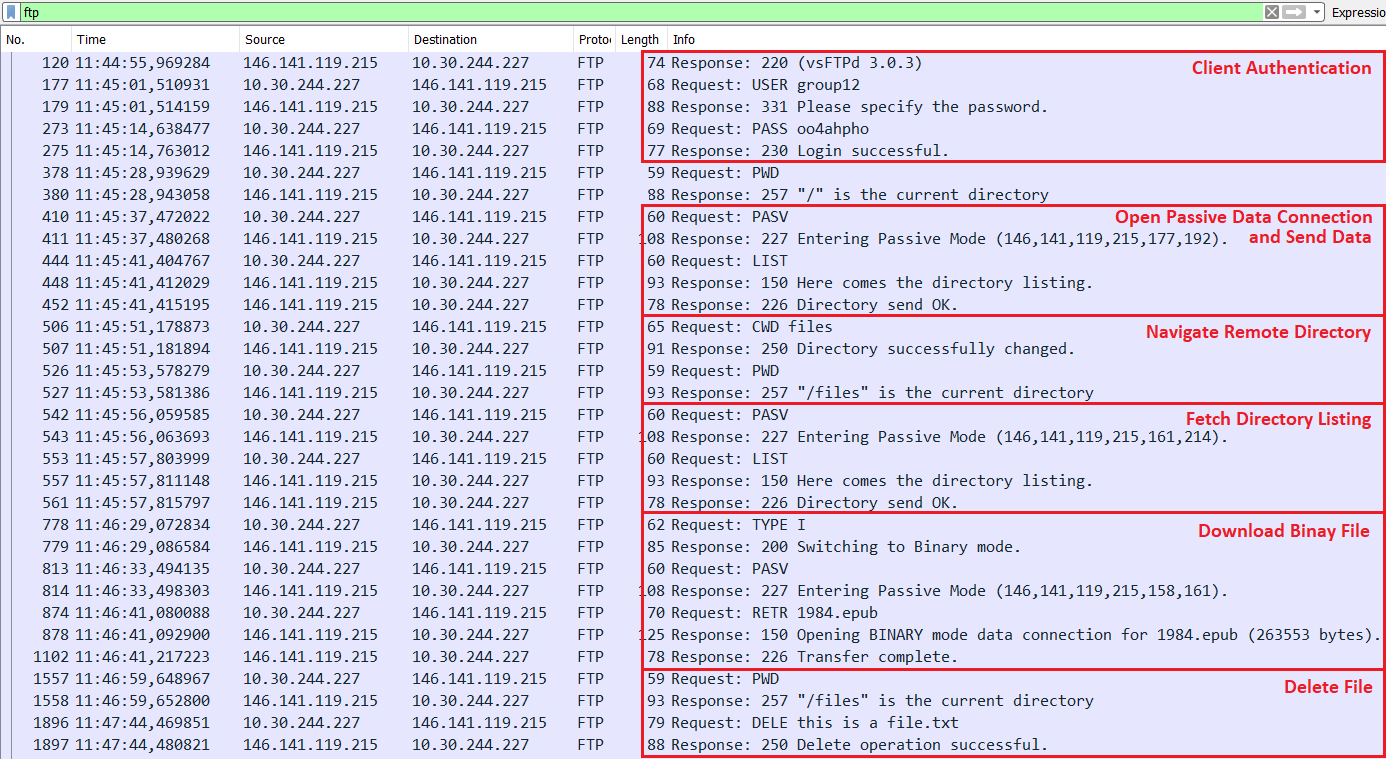
\includegraphics[width=1\columnwidth]{WitsCaptureAnno1.png}
	\caption{Wireshark screenshot of functionality testing with standard FTP server}
	\raggedright
	\label{fig:WitsWS1}
\end{figure}

\begin{figure}[h]
\centering
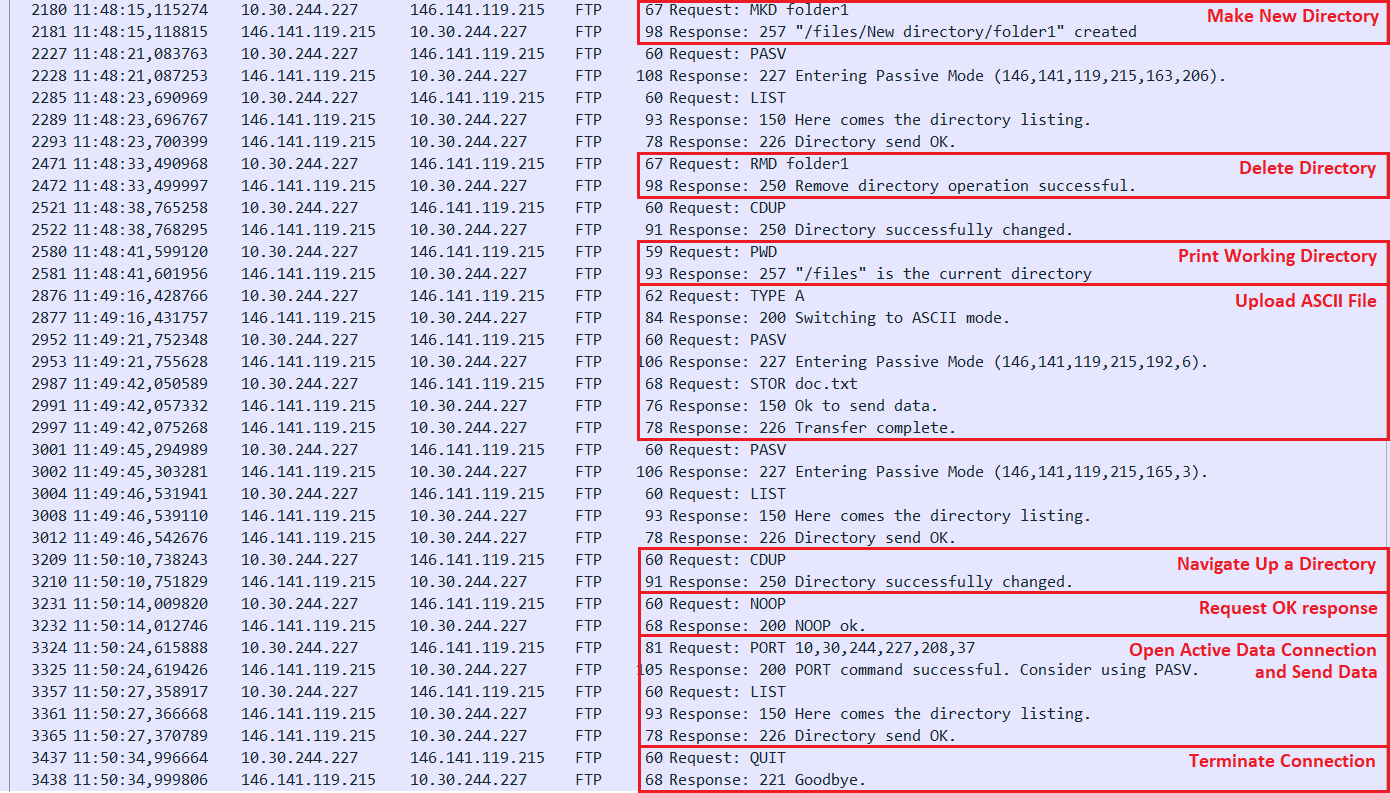
\includegraphics[width=1\columnwidth]{WitsServerCapture2.png}
\caption{captionn}
\raggedright
\label{fig:WitsWS2}
\end{figure}

\end{appendix}

%{\tiny \vfill \hfill \today \hspace{5mm} witseie-paper-2003.\TeX}


\end{document}

" vim: ts=4
" vim: tw=78
" vim: autoindent
" vim: shiftwidth=4
